% Random SVD
\subsection{Randomized SVD}
\label{sec:rsvd}

Randomized SVD is a method to very efficient and effective way to perform approximate singular value decompositions using random matrix theory. The premise is a very large data matrix $\mathbf{X} \in \mathbb{R}^{n \times m}$ that has low \textit{intrinsic rank} $r$, so that $\mathbf{X} \approx \mathbf{U_r \Sigma_r V_r}^T$ will be a good approximation.

\subsubsection{Step 1: Sample Column Space of $\mathbf{X}$ with $\mathbf{P}$}
Given a random projection matrix $\mathbf{P}\in\mathbb{R}^{m \times r}$, the matrix:

\begin{equation}
\mathbf{Z} = \mathbf{XP}
\end{equation}

will, because of the properties of random matrices, likely have the same rank $r$  dominant column space as $\mathbf{X}$. SVD is usually calculated via the QR-decomposition of a matrix. Performing the QR decomposition of $\mathbf{Z}$ is much less laborious, because $\mathbf{Z}\in\mathbb{R}^{m \times r}$ is much smaller than $\mathbf{X}$. We obtain:

\begin{equation}
\mathbf{X} = \mathbf{QR}
\end{equation}

Where $\mathbf{Q}\in\mathbb{R}^{m \times r}$ and $\mathbf{R}\in\mathbb{R}^{r \times r}$.


\subsubsection{Step 2: Compute SVD on Projected $\mathbf{Y = Q^T X}$}
The next step consists of projecting $\mathbf{Z}$ into $\mathbf{Q}$:

\begin{equation}
\mathbf{Y} = \mathbf{Q}^T\mathbf{X}
\end{equation}

Resulting in the matrix $\mathbf{Y}\in\mathbb{R}^{r\times n}$. Performing the SVD on $\mathbf{Y}$ (which is, again, much smaller than $\mathbf{X}$), gives:

\begin{equation}
\mathbf{Y} = \mathbf{U}_Y\mathbf{\Sigma}_r\mathbf{V}_r^T
\end{equation}

Where $\mathbf{\Sigma}_r$ and $\mathbf{V}_r$ turn out to likely be the same as those that would be obtained from the SVD of $\mathbf{X}$ itself. In the last step, $\mathbf{U}_r$ is recovered using the mathrix $\mathbf{Q}$, via $\mathbf{U}_r = \mathbf{QU}_Y$. 

Guaranteed error bounds for the low rank approximation obtained with this technique. There are two approaches to improve the accuracy of randomized SVD. The first is to oversample, by letting the projection matrix $\mathbf{P}$ have a rank larger than $r$. The second is to "sharpen" the singular value spectrum by using the matrix $\mathbf{(X X^T)^q X }$ instead of $\mathbf{X}$. Calculating the power results in a matrix with a much faster drop off in the singular values, but is much more computationally expensive. This technique is useful when the singular values of $\mathbf{X}$ decay only slowly. The column space of the power iteration $\mathbf{...X X^T X X^T X X^T X}$ has the same column space, so that the trick with the projection operation works here too, only that the dominant subspace will be emphasized.\\


\begin{python}
def rSVD(X,r,q,p):
    """
    Randomized SVD Code
    """
    # Step 1: Sample column space of X with P matrix
    ny = X.shape[1]
    P = np.random.randn(ny,r+p)
    Z = X @ P
    for k in range(q):
        Z = X @ (X.T @ Z)

    Q, R = np.linalg.qr(Z,mode='reduced')

    # Step 2: Compute SVD on projected Y = Q.T @ X
    Y = Q.T @ X
    UY, S, VT = np.linalg.svd(Y,full_matrices=False)
    U = Q @ UY

    return U, S, VT
\end{python}

Empirically, randomized SVD outperforms SVD significantly the lower the rank of the TSVD.


\begin{figure}
\centering
    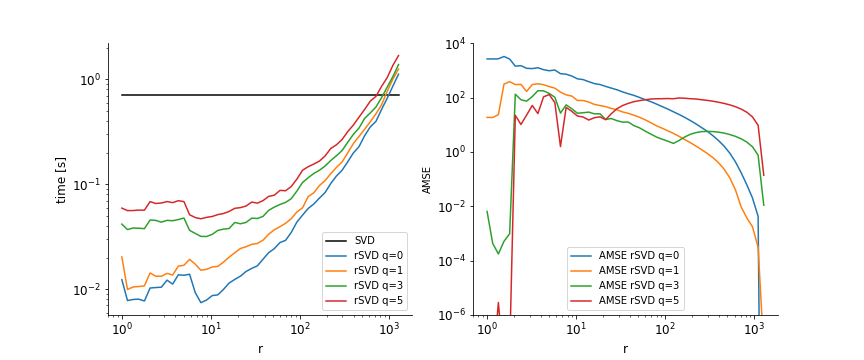
\includegraphics[width=\textwidth]{randomized_svd.png}
    \caption{Left: Time taken to perform conventional SVD (black line) and randomized SVD (colored lines) on the photo of the two young aristocrats which had a data matrix with rank $r=1277$. The different colors correspond to different numbers of power iterations performed ($q$). Right: Average mean square error (AMSE) of truncated SVD using matrices derived with randomized SVD compared with conventional SVD. Especially for small $r$, rSVD is significantly faster even after a few power iterations. For very small $r$, power iterations easily reduce the error introduced by the randomized method by several orders of magnitude, but at some point the method seems to increase the error. Perhaps this is due to numerical stability. I'm not sure. To somewhat account for random fluctuations, the curves shown are averaged over 20 trials.}
    \label{fig:svd_scree}
\end{figure}